%%%% Paramétrage du TD %%%%
\def\xxactivite{Révisions \ifprof -- Corrigé \else \fi} % \normalsize \vspace{-.4cm}
\def\xxauteur{\textsl{Xavier Pessoles}}


\def\xxnumchapitre{Révision \vspace{.2cm}}
\def\xxchapitre{\hspace{.12cm} Résolution des problèmes de statique -- Statique 2D -- Frottement}
\def\xxonglet{\textsf{Rév -- Stat}}
\def\xxactivite{TD 03}
\def\xxauteur{\textsl{Xavier Pessoles}}

\def\xxpied{%
Révision statique -- Frottement sec\\
Fiche 1 -- \xxactivite%
}

\def\xxcompetences{%
\textsl{%
\textbf{Savoirs et compétences :}\\} 
\begin{itemize}
\item \textit{Res2.C18} : principe fondamental de la statique:
\item \textit{Res2.C19} : équilibre d’un solide, d’un ensemble de solides;
\item \textit{Res2.C20} : théorème des actions réciproques.
\end{itemize}
}

\def\xxauteur{\textsl{Xavier Pessoles}}

\def\xxtitreexo{Système EOS \ifnormal $\star$ \else \fi \iftdifficile $\star\star\star$ \else \fi }
\def\xxsourceexo{\hspace{.2cm} \footnotesize{Banque PT SIA -- 2016}}

\def\xxfigures{
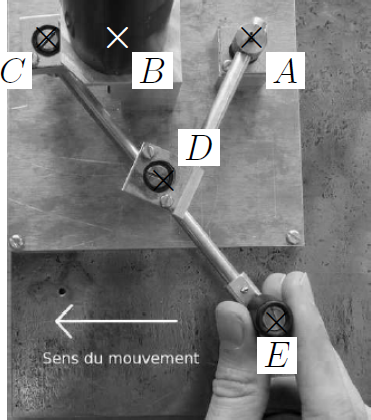
\includegraphics[width=.25\textwidth]{fig_00}
}%figues de la page de garde

